\documentclass[11pt]{article}

\usepackage{times}
\usepackage{epsf}
\usepackage{epsfig}
\usepackage{amsmath, alltt, amssymb, xspace}
\usepackage{wrapfig}
\usepackage{fancyhdr}
\usepackage{url}
\usepackage{verbatim}
\usepackage{fancyvrb}
\usepackage{float}

\usepackage{subfigure}
\usepackage{cite}
\usepackage{hyperref}
\hypersetup{%
    pdfborder = {0 0 0}
}
\topmargin      -0.50in  % distance to headers
\oddsidemargin  0.0in
\evensidemargin 0.0in
\textwidth      6.5in
\textheight     8.9in


%\centerfigcaptionstrue

%\def\baselinestretch{0.95}


\newcommand\discuss[1]{\{\textbf{Discuss:} \textit{#1}\}}
%\newcommand\todo[1]{\vspace{0.1in}\{\textbf{Todo:} \textit{#1}\}\vspace{0.1in}}
\newtheorem{problem}{Problem}[section]
%\newtheorem{theorem}{Theorem}
%\newtheorem{fact}{Fact}
\newtheorem{define}{Definition}[section]
%\newtheorem{analysis}{Analysis}
\newcommand\vspacenoindent{\vspace{0.1in} \noindent}

%\newenvironment{proof}{\noindent {\bf Proof}.}{\hspace*{\fill}~\mbox{\rule[0pt]{1.3ex}{1.3ex}}}
%\newcommand\todo[1]{\vspace{0.1in}\{\textbf{Todo:} \textit{#1}\}\vspace{0.1in}}

%\newcommand\reducespace{\vspace{-0.1in}}
% reduce the space between lines
%\def\baselinestretch{0.95}

\newcommand{\fixmefn}[1]{ \footnote{\sf\ \ \fbox{FIXME} #1} }
\newcommand{\todo}[1]{
\vspace{0.1in}
\fbox{\parbox{6in}{TODO: #1}}
\vspace{0.1in}
}

\newcommand{\mybox}[1]{
\vspace{0.2in}
\noindent
\fbox{\parbox{6.5in}{#1}}
\vspace{0.1in}
}


\newcounter{question}
\setcounter{question}{1}

\newcommand{\myquestion} {{\vspace{0.1in} \noindent \bf Question \arabic{question}:} \addtocounter{question}{1} \,}

\newcommand{\myproblem} {{\noindent \bf Problem \arabic{question}:} \addtocounter{question}{1} \,}



\newcommand{\copyrightnotice}[1]{
\vspace{0.1in}
\fbox{\parbox{6in}{
			This lab was developed by Sparta Global for Cybersecurity courses.
			It was built based on the original lab that was developed for the Labtainer framework by the Naval Postgraduate School, Center for Cybersecurity and Cyber Operations under National Science Foundation Award No. 1438893.
      This work is in the public domain, and cannot be copyrighted.
			}}
\vspace{0.1in}
}


\newcommand{\idea}[1]{
\vspace{0.1in}
{\sf IDEA:\ \ \fbox{\parbox{5in}{#1}}}
\vspace{0.1in}
}

\newcommand{\questionblock}[1]{
\vspace{0.1in}
\fbox{\parbox{6in}{#1}}
\vspace{0.1in}
}


\newcommand{\argmax}[1]{
\begin{minipage}[t]{1.25cm}\parskip-1ex\begin{center}
argmax
#1
\end{center}\end{minipage}
\;
}

\newcommand{\bm}{\boldmath}
\newcommand  {\bx}    {\mbox{\boldmath $x$}}
\newcommand  {\by}    {\mbox{\boldmath $y$}}
\newcommand  {\br}    {\mbox{\boldmath $r$}}


\newcommand{\tstamp}{\today}
%\rfoot[\fancyplain{\tstamp} {\tstamp}]  {\fancyplain{}{}}

\pagestyle{fancy}
\lhead{\bfseries Labtainers}
\chead{}
\rhead{\small \thepage}
\lfoot{\small{\textit{Dr. Osama Abu Oun - Cybersecurity Courses - Sparta Global (\url{https://www.spartaglobal.com/})}}}
\cfoot{}
\rfoot{}

\begin{document}

\begin{center}
{\LARGE IPTables: NAT Rules - Lab Guide}
\vspace{0.1in}\\
\end{center}

\copyrightnotice

\section{Overview}
Iptables is a command line software-based firewall in Linux. It uses policy chains to allow and to block traffic.

IPTables is used as a Firewall and can perform NAT and PAT operations.

In this lab, we focus on IPTables configuration to allow and deny access from/to IP addresses and/or services.

\section{Lab Environment}
This lab runs in the Labtainer framework,
available at http://my.nps.edu/web/c3o/labtainers.
That site includes links to a pre-built virtual machine
that has Labtainers installed, however Labtainers can
be run on any Linux host that supports Docker containers.

From your labtainer-student (~/labtainer/labtainer-student) directory start the lab using:
\begin{verbatim}
    labtainer sparta-nat
\end{verbatim}
\noindent A link to this lab guide will be displayed.

\section{Network Configuration}
IP addresses and routing are configured on all devices.

\begin{figure}[H]
\begin{center}
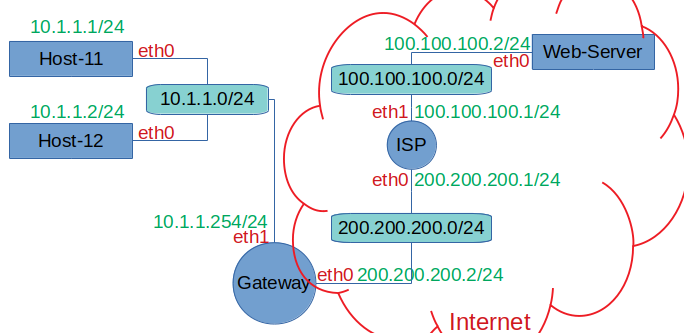
\includegraphics [width=0.8\textwidth]{labtainers-nat-lab-01.png}
\end{center}
\caption{Network topology for routing-basics lab}
\label{fig:topology}
\end{figure}

\section{Credentials}
\begin{itemize}
	\item \textbf{Host-11}:
	\begin{itemize}
		\item \textbf{Username:} user-11
		\item \textbf{Password:} user-11
	\end{itemize}
	\item \textbf{Host-12}:
	\begin{itemize}
		\item \textbf{Username:} user-12
		\item \textbf{Password:} user-12
	\end{itemize}o
	\item \textbf{Web-Server}:
	\begin{itemize}
		\item \textbf{Username:} web-admin
		\item \textbf{Password:} web-admin
	\end{itemize}
	\item \textbf{Firewall}:
	\begin{itemize}
		\item \textbf{Username:} admin
		\item \textbf{Password:} admin
	\end{itemize}
\end{itemize}

\section{Lab Tasks}

\subsection{Testing the Initial Configuration}\label{Testing the Initial Configuration}
Lets check what we can/can't do in this network.
\newline
\begin{itemize}
	\item On Host-11 (Ping Host-11 -$>$ Gateway: Internal Interface)
	\begin{verbatim}
	    ping 10.1.1.254
	\end{verbatim}

	What is the result ?

	\item On Host-11 (Ping Host-11 -$>$ Gateway: External Interface)
	\begin{verbatim}
	    ping 200.200.200.2
	\end{verbatim}

	What is the result ?

	\item On Host-11 (Ping Host-11 -$>$ ISP: eth0)
	\begin{verbatim}
	    ping 200.200.200.1
	\end{verbatim}

	What is the result ?

\end{itemize}

\subsection{Capturing the Traffic}
Lets use \textbf{tcpdump} which is a command line tool that can capture TCP/IP and other packets being transmitted or received over a network interface.
\newline
\newline
In the ISP terminal, run the following command:
\begin{verbatim}
    sudo tcpdump -i eth0
\end{verbatim}

\textbf{eth0} is the interface connected to our gateway. You can make sure of that by running \textbf{ifconfig} or \textbf{ip add}
\newline
\newline
Now, you can see that the packets are arriving at the ISP router (with their private IP address), but then the ISP router has no routes for private IP addresses that they exist in customers networks so it doesn't know where to send the response.

\subsection{Testing the Initial Configuration}\label{Testing the Initial Configuration}
\begin{itemize}
	\item On Host-11 (Send HTTP request Host-11 -$>$ Web-Server to get a web page)
	\begin{verbatim}
	    wget http://10.1.2.1/index.html
	\end{verbatim}

	What is the result ?

	\item Check the router terminal, scroll up to check all the packets captured by the router. Notice that you can find the content of the html page.

		That means the traffic isn't encrypted and the packets (info) can be read by any device on the route between the client and the server.
\end{itemize}
\subsection{Configuring the NAT Rules on the Firewall}
Lets run this command that will perform NAT on all packets passing by the gateway and leaving the router from the interface `eth0` which is the interface connected to the ISP router in our design and it has the public IP address which is the routable address in the network.

\begin{verbatim}
		sudo iptables -t nat -A POSTROUTING -o eth0 -j MASQUERADE
\end{verbatim}

Now, stop the ping command on Host-11 and re-issue the command again, notice that the ping is working and the ISP router is receiving the packets with the public IP address of the router rather than the private IP address of the host itself.
\newline
\newline
Repeat the same command from host-12 and notice that the router is receiving the packets from the Host-12 with the gateway public IP address too.
\newline
\newline
In a way, the ISP router cannot tell which host is sending these packets.

Try fetching the web page from the web server using wget
\begin{itemize}
	\item Test the connectivity: On Host-11 (Send HTTP request Host-11 -$>$ Web-Server to get a web page)
	\begin{verbatim}
			wget http://100.100.100.2/index.html
	\end{verbatim}

	What is the result ?

	\item Test the connectivity: On Host-11 (Send HTTP request Host-11 -$>$ Web-Server to get a web page)
	\begin{verbatim}
			wget http://100.100.100.2/index.html
	\end{verbatim}

	What is the result ?
\end{itemize}

\section{Submission}
After finishing the lab, go to the terminal on your Linux system that was used to start the lab and type:
\begin{verbatim}
    stoplab sparta-nat
\end{verbatim}
When you stop the lab, the system will display a path to the zipped lab results on your Linux system.  Provide that file to
your instructor, e.g., via the Sakai site.

\end{document}
